\documentclass[11pt,a4paper]{article}
\usepackage{amsmath}
\usepackage{amsfonts}
\usepackage{amssymb}
\usepackage{fancyhdr}
\usepackage{lastpage}
\usepackage{graphicx}
\usepackage{ucs}
\usepackage[utf8x]{inputenc}
\usepackage[italian]{babel}
\usepackage[colorlinks=true,linkcolor=black]{hyperref}

\renewcommand{\headrulewidth}{0.6pt}
\renewcommand{\footrulewidth}{0.6pt}
% impostazione dello stile per le pagine interne del documento
\lhead{\leftmark}
\chead{}
\rhead{
\includegraphics[scale=0.15]{logo.png} }
\lfoot{Definizione di prodotto v0.2.0}
\cfoot{}
\rfoot{\thepage \ di \pageref{LastPage}}
% ridefinizione dello stile plain per il frontespizio
\fancypagestyle{plain}{
\fancyhf
}
% impostazione dello stile per l'indice
\fancypagestyle{indice}{
\lhead{\leftmark}
\chead{}
\rhead{
\includegraphics[scale=0.15]{logo.png}}
\lfoot{Definizione di prodotto v0.2.0}
\cfoot{}
\rfoot{}
}
\headheight = 46pt
%definizione del comando "\modfiche" per la creazione del diario delle modifiche
\newcommand{\modifiche} 
{
\newpage
\begin{center}
\textbf{Diario delle modifiche} \\
\bigskip
\begin{tabular}{|c|c|p{0.51\textwidth}|}
\hline
\textsc{Data} & \textsc{Versione} & \textsc{Modifica} \\
\hline
\hline
\textit{4 marzo 2009} & 0.2.0 & Stesura parte sul componente MiddleMan \\
\hline
\textit{20 febbraio 2009} & 0.1.0 & Stesura dell'indice \\
\hline
\end{tabular}
\end{center}
}
%definizione del comando "\info" per la creazione delle informazioni del documento
\newcommand{\info} {
\bigskip
\begin{tabbing}
	\hspace*{0.3\textwidth} \= \hspace*{0.5\textwidth} \kill
	\parbox{0.3\textwidth}{\textbf{Verifica: }} \> \parbox{0.5\textwidth}{Verificatore} \\
	\parbox{0.3\textwidth}{\textbf{Approvazione: }} \> \parbox{0.5\textwidth}{Responsabile} \\
	\parbox{0.3\textwidth}{\textbf{Stato: }} \> \parbox{0.5\textwidth}{Preliminare | Formale} \\
	\parbox{0.3\textwidth}{\textbf{Uso: }} \> \parbox{0.5\textwidth}{Interno | Esterno} \\
	\parbox{0.3\textwidth}{\textbf{Distribuzione: }} \> \parbox{0.5\textwidth}{QuiXoft} \\
\end{tabbing}
}
%definizione del comando "\frontespizio" per la creazione del frontespizio
\newcommand{\frontespizio} {
\thispagestyle{plain}
\title{\begin{Huge}\textsc{Progetto SIGEOL}\end{Huge} \\ \textit{Definizione di prodotto \\ v0.2.0}}
\author{Redazione: }
\maketitle
\medskip
\begin{center}

\includegraphics[scale=0.5]{logo.png} \\
\textit{quixoft.sol@gmail.com}
\end{center}
\medskip
\info
\begin{center}
\textbf{Sommario} \\
Descrizione dettagliata delle caratteristiche tecniche ed architetturali del prodotto \textsc{Sigeol}
\end{center}
\newpage
}
%definizione del comando "\indice" per la creazione dell'indice
\newcommand{\indice} {
\thispagestyle{indice}
\tableofcontents
\newpage
}
\pagestyle{fancy}
\begin{document}
\frontespizio
\indice
\setcounter{page}{1}
\section{Introduzione}
\subsection{Scopo del documento}
Il presente documento denominato \textsc{Descrizione di prodotto} si prefigge di illustrare ed analizzare con maggior dettaglio i metodi ed i formalismi adottati nella definizione del prodotto \textsc{Sigeol}
\subsection{Scopo del prodotto}
Il progetto sotto analisi, denominato \textsc{Sigeol}, si prefigge di automatizzare la generazione, la gestione, l’ottimizzazione e la consultazione degli orari di lezione. Per maggiori dettagli consultare il documento denominato \textsc{Analisi dei Requisiti} alla sua ultima versione.
\subsection{Glossario}
Le definizioni dei termini specialistici usati nella stesura di questo e di tutti gli altri documenti possono essere trovate nel documento denominato \textsc{Glossario} al fine di eliminare ogni ambiguità e di facilitare la comprensione dei temi trattati. Ogni termine la cui definizione è disponibile all’interno del glossario verrà marcato con una sottolineatura.
\subsection{Riferimenti normativi}
Il documento denominato \textsc{Norme di Progetto} accompagna e complementa il presente ed ogni documento ufficiale.

\section{Standard di progetto}
\subsection{Standard di progettazione architetturale}
La definizione dell'intero sistema oggetto di studio è stata effetuata attraverso l'uso di diagrammi UML e l'applicazione di pattern consolidati ed in uso in molti prodotti software.
\subsubsection{UML}
Il linguaggio UML è utilizzato per la modellazione architetturale di un sistema in quanto grazie alla sua capacità e chiarezza espressiva risulta di facile comprensione anche a persone esterne al progetto stesso. Il team QuiXoft ha utilizzato UML 2.0 per:
\begin{itemize}
 \item Diagrammi use-case nel documento \textsc{Analisi dei Requisiti}
 \item Diagrammi delle classi, delle componenti, di attività e delle sequenze nei documenti \textsc{Specifica tecnica} e \textsc{Definizione di prodotto}
\end{itemize}
\subsection{Pattern}
All'interno dell'architettura del sistema sono stati utilizzati i seguenti pattern, presenti nel \underline{framework} Ruby on Rails il quale è alla base di tutto il prodotto:
\begin{description}
 \item[\textbf{MVC}] 
Il \underline{pattern} MVC (Model View Controller) si basa sulla separazione tra i componenti software del sistema, che gestiscono il modo in cui presentare i dati, e i componenti che gestiscono i dati stessi. 
 \item[\textbf{Façade}]
Permette, attraverso un'interfaccia più semplice, l'accesso a sottosistemi aventi interfacce complesse e molto diverse tra loro, nonché a blocchi di codice complessi.
\item[\textbf{REST}]
Representational state transfer (REST) è un tipo di architettura software per i sistemi di ipertesto distribuiti come il World Wide Web. 
REST si riferisce ad un insieme di principi di architetture di rete, i quali delineano come le risorse sono definite e indirizzate.

\item[\textbf{Convention Over Configuration}]
Convention Over Configuration è un paradigma di programmazione che prevede configurazione minima (o addirittura assente) per il programmatore che utilizza un \underline{framework} che lo rispetti, obbligandolo a configurare solo gli aspetti che si differenziano dalle implementazioni standard o che non rispettano particolari convenzioni di denominazione o simili.
Significa che Rails prevede delle impostazioni di default per qualsiasi aspetto dell’applicazione. Utilizzando queste convenzioni sarà possibile velocizzare i tempi di sviluppo evitando di realizzare scomodi file di configurazione. L’esempio più chiaro del COC si può notare a livello di modelli: rispettando le convenzioni previste dal \underline{framework} è possibile realizzare strutture di dati complesse con molte relazioni tra oggetti in pochissimo tempo, in maniera quasi meccanica e soprattutto senza definire nessuna configurazione. Questo concetto differenzia Rails dai \underline{framework} che prevedono molte righe di configurazione per ogni aspetto dell’applicazione. Con il COC tutto diventa più snello e più dinamico. Ovviamente per situazioni in cui le convenzioni non possano essere rispettate, Rails permette di utilizzare schemi funzionali diversi da quelli previsti.
\item[\textbf{DRY}]
Questo concetto, fortemente filosofico, prevede che ciascun elemento di un’applicazione debba essere implementato solamente una volta e niente debba essere ripetuto. Questo significa che, mediante Rails, è possibile gestire funzionalità ripetitive con una estrema fattorizzazione del codice (''scrivo una volta e uso più volte'') che facilita sia lo sviluppo iniziale che eventuali modifiche successive del prodotto.
\item[\textbf{View Helper}]
Questo \underline{pattern} disaccoppia il Business Logic dallo strato View, il che facilita
la manutenibilità. Aiuta a separare, in fase di sviluppo, la responsabilità
del web designer e dello sviluppatore.
\item[\textbf{Active Record}]
Secondo il \underline{pattern} Active Record esiste una relazione molto stretta fra tabella e classe, colonne e attributi della classe. 
\begin{itemize}
 \item una tabella di un \underline{database} relazionale è gestita attraverso una classe
\item una singola istanza della classe corrisponde ad una riga della tabella
\item alla creazione di una nuova istanza viene creata una nuova riga all'interno della tabella, e modificando l'istanza la riga viene aggiornata
\end{itemize}
\end{description}

\subsection{Standard di documentazione del codice}
Il team QuiXoft si avvalerà dello strumento \underline{RDoc}, specifico per il linguaggio Ruby. Questo strumento estrapola dal codice sorgente i commenti al codice stesso, organizzandoli e rendendoli disponibili alla consultazione tramite pagine HTML. Per questo motivo ogni membro del team alla stesura di qualsiasi classe o metodo dovrà documentarlo tramite la sintassi specifica di RDoc.

\subsection{Standard di denominazione di entità e relazioni}
Lo schema di denominazione deve essere determinante per la comprensione del flusso logico dell'applicazione. Verrano quindi utilizzati nomi significativi che identifichino la funzione e lo scopo dell'elemento. Inoltre saranno seguite le convenzioni generali dello specifico linguaggio di programmazione utilizzato per realizzare l'elemento, nonchè ulteriori convenzioni dettate dal framework utilizzato. Per maggiori informazioni consultare la sezione \ref{programmazione}

\subsection{Standard di programmazione}\label{programmazione}
Ogni file deve contenere esattamente una classe od un modulo, eccezion fatta per i \underline{template} di file HTML e JavaScript. Inoltre è necessaria ai fini di una migliore leggibilità, l'uso di una corretta indentazione, fornita dall'ambiente di sviluppo. 
\subsubsection{Ruby e framework Rails}
Di seguito sono elencate le convenzioni utilizzate negli elementi sviluppati con il linguaggio Ruby.
\subsubsection*{Variabili locali}
Prima lettera minuscola, seguita da altri caratteri minuscoli. Se la variabile comprende più parole, queste andranno separate con un \_ (underscore). Esempio: \verb|variabile_locale|
\subsubsection*{Variabili d'instanza}
Si utilizza la stessa convenzione adottata nelle variabili locali, con l'aggiunta di un @ (at) prima del nome. Esempio: \verb|@variabile_istanza|
\subsubsection*{Variabili di classe}
Si utilizza la stessa convenzione adottata nelle variabili locali, con l'aggiunta di una doppia @ (at) prima del nome. Esempio: \verb|@@variabile_classe|
\subsubsection*{Variabili globali}
Si utilizza la stessa convenzione adottata nella variabili locali, con l'aggiunta di un \verb|$| (dollar) prima del nome. Esempio: \verb|$variabile_globale|
\subsubsection*{Costanti}
Prima lettera maiuscola, seguita da altri caratteri maiuscoli. Se la variabile comprende più parole, queste andranno separate con un \_ (underscore). Esempio: \verb|UNA_COSTANTE|
\subsubsection*{Metodi d'istanza}
Prima lettera minuscola, seguita da altri caratteri minuscoli. Se il nome comprende più parole, queste andranno separate con un \_ (underscore). Esempio: \verb|metodo_istanza|
\subsubsection*{Classi e moduli}
Prima lettera maiuscola, seguita da altri caratteri minuscoli. Se il nome comprende più parole, la prima lettera di ogni parola deve essere maiuscola. Esempio: \verb|UnaClasse|
\subsubsection*{Model}
Si utilizza la stessa convenzione per le classi ed inoltre il nome dovrà essere il singolare (in lingua inglese) del nome della tabella del database a cui si riferisce. Esempio: \verb|Order|
\subsubsection*{Controller}
Si utilizza la stessa convenzione per le classi ed inoltre il nome dovrà essere il plurale (in lingua inglese) del nome del Model a cui si riferisce, seguito dalla parola \textit{Controller}. Esempio: \verb|OrdersController|
\subsubsection*{Tabelle del database}
Prima lettera minuscola, seguita da altri caratteri minuscoli. Se il nome comprende più parola, queste andranno separate con un \_ (underscore). Inoltre il nome deve essere il plurale del model (in lingua inglese) a cui la tabella si riferisce. Esempio: \verb|orders|
\subsubsection*{Chiave primaria}
Il nome della chiave primaria dovrà essere \verb|id|
\subsubsection*{Chiavi esterne}
Il nome della chiave esterna dovrà essere il singolare (in lingua inglese) della tabella di riferimento, seguito da un \_ (underscore) e dalla parola \textit{id}, con ogni carattere minuscolo. Esempio: \verb|order_id|
\subsubsection*{Tabelle per le relazioni molti a molti}
Concatenazione tramite \_ (underscore) dei nomi al plurale (in lingua inglese) dei model coinvolti in ordine alfabetico, con ogni carattere minuscolo. Esempio \verb|items_orders|
\subsubsection*{File}
Ogni nome di file è caratterizzato dalla presenza di soli caratteri minuscoli e la concatenazione di più parole è effettuata tramite \_ (underscore).
\subsubsection{Java}
Per quanto riguarda i file sorgenti scritti utilizzando il linguaggio Java fanno fede le norme e convenzioni acquisite da ogni membro del team durante il corso di Programmazione 3 o Programmazione concorrente e distribuita, a seconda dell'ordinamento a cui il componente appartiene.

\subsection{Strumenti di lavoro}
Durante tutto lo svolgimento del progetto, il team QuiXoft utilizzarà i seguenti strumenti:
\begin{itemize}
 \item IDE NetBeans 6.5 \\ \textit{http://www.netbeans.org/}
 \item JDK 6 Update 12 \\ \textit{http://java.sun.com/}
 \item JRuby 1.1.5 \\ \textit{http://jruby.codehaus.org/}
 \item GlassFishV3 \\ \textit{https://glassfish.dev.java.net/}
 \item MySql 5.0 \\ \textit{http://www.mysql.com/}
 \item Rails framework \\ \textit{http://rubyonrails.org/}
 \item RDoc \\ \textit{http://rdoc.sourceforge.net/}
 \item rcov \\ \textit{http://rubyforge.org/projects/rcov/}
 \item W3C validator \\ \textit {http://validator.w3.org/}
 \item Prototype 1.6 \\ \textit {http://www.prototypejs.org/}
 \item \LaTeX \\ \textit {http://www.latex-project.org/}
\end{itemize}

\section{Specifica delle componenti}
Il sistema Sigeol è strutturato seguendo il paradigma MVC, con l'aggiunta di ulteriori: Helper, MiddleMan e Algorithm.
\subsection{Componente Model}\label{model}
\subsubsection{Introduzione}
Ogni classe appartente al model, è una sottoclasse, della classe \verb|Base|, presente nella cartella \verb|active_record|.


Quando una classe deriva da \verb|Base|, il suo oggetto istanziato viene anche chiamato oggetto di tipo Active Record.
In un oggetto di questo tipo, gli attributi non vengono specificati direttamente, ma vengono dedotti dalla tabella associata.


In rails, per poter associare una classe Active Record ad una tabella, si devono seguire queste convenzioni:
\begin{itemize}
 \item la tabella deve essere chiamata con un nome plurale e tutto in minuscolo
 \item la classe deve essere chiamata con lo stesso nome della tabella, ma al singolare e con la prima lettera maiuscola
\end{itemize}
Quindi se si crea una tabella users la classe del model dovrà essere chiamata User.


Un'istanza di una classe del model corrisponde ad una riga della tabella associata.
Se viene cancellato un oggetto model, verrà cancellata anche la riga corrispondente.


Da \verb|base| si ereditano diversi metodi tra i quali:
\begin{itemize}
 \item \verb|save|: salva l'oggetto model. Se il model è nuovo viene creato un record nel database, altrimenti il record esistente viene aggiornato.
 \item \verb|destroy|: elimina il record associato. Ovviamente dopo questa operazione l'oggetto model corrispondente alla riga cancellata, non potrà più modificare gli attributi.
\end{itemize}
\paragraph{Validazioni}
Grazie alla libreria \verb|Active Record| è possibile validare gli attributi di un oggetto model. La validazione viene eseguita automaticamente prima di creare il record nel database. Se la convalida fallisce, l'oggetto non verrà scritto nel db e verrà lasciato in memoria.


\verb|Active record| distingue i models che corrispondono ad un record esistente e quelli che non lo sono. Quando viene chiamato il metodo \verb|save|, \verb|Active Record| effettuerà un operazione SQL di Insert per i nuovi record e un update per le righe esistenti. Grazie a questo, è possibile specificare quando effettuare le validazioni (prima di aggiornare il record, prima di crearlo od ogni volta che lo si salva).


\verb|Active record|, ha un set di helpers methods che implementano delle validazioni comuni a molti models; per esempio il controllo che il contenuto dell'attributo non sia nullo.
Se il controllo fallisce, verrà aggiunto un messaggio di errore all'attributo che non soddisfa la validazione e l'oggetto non verrà salvato.
Ad esempio nel model \verb|User|, per controllare la presenza dell'attributo \verb|mail|, si utilizza l'helper method 
\begin{center}
 \verb|validates_presence_of:|\\
 \verb|:message=>"La mail non deve essere vuota"|\\
 \verb|:on  => :update|\\
\end{center}
dove \verb|:message| contiene il messaggio d'errore e \verb|:on| specifica quando effettuare la validazione(\verb|:create|, \verb|:update|).

 
Se \verb|:on| è omesso la validazione verrà fatta prima di ogni chiamata del metodo save.


Infine, per creare una validazione, è necessario aggiungere alle chiamate di \verb|validate|, \verb|validate_on_update|,\verb|validate_on_create|, la lista dei metodi(passati come simboli) che si vuole eseguire.
\begin{itemize}
 \item \verb|validate|: la validazione viene eseguita prima di ogni operazione di scrittura nel database; quindi sia in fase di creazione che di modifica
 \item \verb|validate_on_create|:la validazione viene eseguita solo quando\\ un nuovo model dev'essere salvato nel database
 \item \verb|validate_on_update|:la validazione viene eseguita solamente quando si modifica una riga già esistente
\end{itemize}


Ad esempio, nel model \verb|ExpiryDate|, per controllare che la data immessa sia maggiore di quella di oggi si è implementato il \\metodo \verb|is_correct_date?|
Il nome poi è stato aggiunto come simbolo alla chiamata di \verb|validate| in questo modo: \verb|validate :is_correct_date?|


Ora, un qualsiasi oggetto di tipo \verb|ExpiryDate| è valido solo se contiene una data maggiore della data di oggi.
\paragraph{Associazioni}
Oltre alle validazioni, nelle classi del model sono definite le relazione tra le tabelle.
\verb|Active record| supporta tre tipi di associazioni: one-to-one, one-to-many, many-to-many.
Per dichiarare una relazione, basta inserire opportunamente nelle classi del model: \verb|has_one|, \verb|has_many|, \verb|belongs_to| e \verb|has_and_belongs_to_many|.
Anche qui è necessario seguire delle convenizioni:
\begin{itemize}
 \item la dichiarazione di \verb|belongs_to| deve essere aggiunta nel model della tabella che contiene la chiave esterna
 \item dopo \verb|has_many| e \verb|has_and_belongs_to_many| deve essere aggiunto come simbolo il nome della tabella
 \item dopo \verb|belongs_to| e \verb|has_one| deve essere aggiunto come simbolo il nome al singolare della tabella
\end{itemize}



E' possibile modificare le associazioni aggiungendo delle opzioni; in particolare nel progetto \textit{Sigeol} si è utilizzata l'opzione :dependent.
Questa indica ad \verb|Active record| come comportarsi quando si elimina una riga del parent table rispetto al child table.
Ad esempio nel model GraduateCourse la relazione con la tabella curriculums è definita in questo modo:\\
\verb|has_many :curriculums, :dependent => :destroy|
Cancellando una riga di \verb|graduate_courses|, verranno cancellate tutte le righe associate di \verb|curriculums|.

\paragraph{Associazioni polimorfe}
Nel progetto \textit{Sigeol} sono presenti due associazioni polimorfe.


La prima è tra il model \verb|User|, \verb|Teacher| e \verb|DidacticOffice|.\\ 
Per implementare quest'associazione, si è aggiunto alla tabella \verb|users| due attributi: \verb|specified_id| e \verb|specified_type|.
Ora nel model \verb|User| è necessario specificare che si sta creando un'associazione polimorfa attraverso \verb|specified_id| e \verb|specified_type|:\\
\verb|belongs_to :specified, :polymorphic => true|.\\
Ora nei tipi che può assumere User(Model \verb|Teacher| e \verb|DidacticOffice| si specifica questa associazione:\\
\verb|has_one :user, :as => :specified|\\
L'opzione \verb|:as=>specified|, specifica che la relazione tra \verb|User| e il model che contiene l'associazione definita sopra è polimorfa, usando l'attributo specified.


Ad esempio, sia u un oggetto di tipo \verb|User| e t un oggetto di tipo \verb|Teacher|, per specificare lo user, semplicemente basta fare:\\
\verb|u.specified=t|

Il secondo tipo di associazione è chiamata \textit{associazione polimorfa doppia}\\ 
A parole, il problema si può spiegare in questo modo: una corso di laurea o una classe, possono avere più vincoli di diverso tipo; ad esempio possono avere due vincoli di tipo temporale ed uno di quantità. A sua volta un vincolo può avere più tipi di proprietari: una classe, un insegnante o un corso di laurea.
Insomma, un vincolo può avere più tipi di proprietari e un proprietario può avere più tipi di vincoli; questa situazione si chiama 
Per implementare questa associazione si farà uso di un plugin chiamato :\verb|has_many_polymorphs|. 


Inoltre si dovrà aggiungere una nuova classe che associerà tutti i tipi di vincoli con tutti i tipi di proprietari. Questo tipo di model è chiamato join model




\paragraph{Funzioni di callback}
\verb|ActiveRecord| mette a disposizione dei metodi che monitorano lo stato dell'oggetto. 
E' possibile quindi definire delle operazioni da eseguire prima o dopo l'alterazione dello stato dell'oggetto.


Ad esempio, per eseguire un metodo prima di effettuare le validazioni, basterà chiamare la funzione di callback \verb|before_validation|, seguita dal nome, passato come simbolo, del metodo che si vuole eseguire.
Oltre a \verb|before_validation| sono presenti altre funzioni come \verb|before_create|, \verb|before_destroy|, \verb|after_create|...  

\subsection{Descrizione dei models}
Nella descrizione delle validazioni, verrà omessa la parte di codice che mostra le opzioni; tuttavia queste sono facilmente intuibili dalla descrizione.
\subsubsection{AcademicOrganization}
\paragraph{Validazioni}
\begin{itemize}
 \item \verb|validates_uniqueness_of :name|:\\ valida che nella tabella \verb|academic_organizations| non sia presente nessuna riga con lo stesso valore dell'attributo \verb|name| 
\item \verb|validates_presence_of :name|: valida che il contenuto di \verb|name| non sia vuoto
\item \verb|validates_length_of :name:maximum => 30|: il contenuto di \verb|name| deve essere al massimo di 30 caratteri
\item \verb|validates_format_of :name:with => /^[a-zA-Zàòèéùì\s]*$/|: il valore di \verb|name| deve rispettare l'espressione regolare. Per essere valido \verb|name| dovrà contenere solo caratteri maiuscoli, minuscoli, spazi e lettere accentate.
\item \verb|validates_uniqueness_of :number|:\\ valida che nella tabella \verb|academic_organizations| non sia presente nessuna riga con lo stesso valore dell'attributo \verb|number|
 \item \verb|validates_numericality_of :number|: il contenuto di \verb|number| deve essere un intero compreso tra 1 e 6
\end{itemize}
\paragraph{Funzioni di callback}
\subparagraph{before\_validation}
\begin{center}
 \verb|def before_validation|\\
   \verb|self.name=first\_upper(self.name)|\\
 \verb|end|
\end{center}
Prima di effettuare le operazioni di validazione, il contenuto dell'attributo \verb|name| viene messo tutto in minuscolo, tranne la prima lettera che viene messa in maiuscolo. 
\paragraph{associazioni}
\begin{itemize}
\item \verb|has_many :graduate_courses|: \\tra \verb|academic_organizations| e \verb|graduate_courses| esiste un'associziazione di tipo one-to-many. 
\end{itemize}
\subsubsection{Address}
\paragraph{Validazioni}
Le validazioni di \verb|city| e di \verb|street| sono identiche all'attributo \verb|name| del model \verb|AcademicOrganization|, senza però il controllo dell'unicità tramite \verb|:validate_uniqueness|
\begin{itemize}
 \item \verb|validates_length_of :telephone, :maximum => 13|: il numero di telefono deve essere al massimo di 13 caratteri
 \item \verb|validates_format_of :telephone,|\\ 
      \verb|:with => /^[0-9]{2,4}-[0-9]{6,8}$/|:\\ il contenuto di \verb|telephone| deve rispettare l'espressione regolare. Per essere valido, \verb|telephone| deve avere un numero di cifre compreso tra due e quattro(prefisso), seguite dal simbolo - ed infine un secondo numero di cifre compreso tra sei e otto(numero di telefono). Non è necessario inserire e controllare prima del numero di telefono il prefisso internazionale, perchè si ipotizza che tutti i numeri inseriti siano italiani.
\end{itemize}
\paragraph{Funzioni di callback}
\subparagraph{before\_save}
Prima di salvare l'oggetto nel database, il contenuto degli attributi \verb|city| e \verb|street| vengono messi in minuscolo, tranne la prima lettera che viene messa in maiuscolo. Il codice è simile a quello presente nella funzione \verb|before_validation| del model \verb|AcademicOrganization| 
\paragraph{Associazioni}
\begin{itemize}
 \item \verb|has_one :user|: si sta definendo una relazione one-to-one con il model \verb|User|. 
 \item \verb|has_one :building|: si sta definendo una relazione one-to-one con il model \verb|Building|.
\end{itemize}
\subsubsection{Belong}
\paragraph{Descrizione attributi}
\begin{itemize}
 \item \verb|curriculum_id|: chiave esterna di curriculums
 \item \verb|teaching_id|: chiave esterna di teachings
 \item \verb|isOptional|: è un attributo booleano. Se settato a true, indica che l'insegnamento individuato dalla chiave esterna \verb|teaching_id|, è opzionale rispetto al curriculum individuato della chiave esterna \verb|curriculum_id|	
\end{itemize}
\paragraph{Validazioni}
\begin{itemize}
 \item \verb|validates_presence_of :curriculum_id|: valida che il contenuto della chiave esterna \verb|curriculum_id| non sia nullo. 
 \item \verb|validates_presence_of :teaching_id|: valida che il contenuto della chiave esterna \verb|teaching_id| non sia nullo
\end{itemize}
\subparagraph{validate\_on\_create}
\begin{itemize}
 \item \verb|validate_on_create :unique_curriculum_id_and_teaching_id?|: \\E' possibile salvare nel database l'oggetto istanziato, solo se nessuna riga della tabella associata \verb|belongs|, ha gli stessi valori di \verb|teaching_id| e di \verb|curriculum_id| dell'istanza.\\
 \verb|unique_curriculum_id_and_teaching_id?| è un metodo privato.
\end{itemize}
\paragraph{Funzioni di callback}
\subparagraph{before\_destroy}
\begin{center}
\verb|def after_destroy|\\
    \verb|if(Belong.count)|
    \verb|(:conditions=>["teaching_id = ?" , self.teaching_id])==0)|\\
      \verb|Teaching.destroy(teaching_id)|\\
    \verb|end|\\
  \verb|end|
\end{center}
Dopo aver eliminato l'oggetto, se nessun curriculum utilizza l'insegnamento(associato all'istanza appena cancellata), allora anch'esso verrà cancellato.
\paragraph{Associazioni}
\begin{itemize}
 \item \verb|belongs_to :teaching|: tra \verb|teachings| e \verb|belongs| esiste un'associazione one-to-many; \verb|belongs| contiene la chiave esterna
 \item \verb|belongs_to :curriculum|: tra \verb|curriculums| e \verb|belongs| esiste un'associazione one-to-many; \verb|belongs| contiene la chiave esterna 	
\end{itemize}
\subsubsection{Building}
\paragraph{Descrizione attributi}
\begin{itemize}
 \item \verb|name|: contiene il nome del palazzo
 \item \verb|address_id|: chiave esterna di addresses	
\end{itemize}
\paragraph{Validazioni}
Le validazioni di \verb|name| sono identiche all'attributo \verb|name| del model \verb|AcademicOrganization|
\begin{itemize}
 \item \verb|validates_presence_of :address_id|: valida che il contenuto della chiave esterna non sia vuoto
\end{itemize}
\paragraph{Funzioni di callback}
\subparagraph{before\_validation}
Prima di validare l'oggetto, il contenuto di \verb|name| viene messo in minuscolo, tranne la prima lettera che viene messa in maiuscolo. Per il codice, vedere la sezione \verb|before_validation|\\ di \verb|AcademicOrganization| 
\paragraph{Associazioni}
\begin{itemize}
 \item \verb|belongs_to :address, :dependent => :destroy|: tra \verb|addresses| e \verb|buildings| esiste un'associazione one-to-one; \verb|buildings| contiene la chiave esterna. Se viene eliminato un building, viene eliminato anche il suo address associato
 \item \verb|has_many :classrooms, :dependent => :destroy|:\\ tra \verb|classrooms| e \verb|buildings| esiste un'associazione one-to-many. Se viene eliminato un building, vengono anche eliminate tutte le sue classrooms associate.
\end{itemize}
\subsubsection{Capability}
\paragraph{Descrizione attributi}
\begin{itemize}
 \item \verb|name|: contiene il nome del servizio, disponibile per gli utenti del sistema
\end{itemize}
\paragraph{Validazioni}
Le validazioni di \verb|name| sono identiche all'attributo \verb|name| del model \verb|AcademicOrganization|
\paragraph{Associazioni}
\begin{itemize}
 \item \verb|has_and_belongs_to_many :users|: tra \verb|capabilities| e \verb|users| esiste un'associazione many-to-many
\end{itemize}
\subsubsection{Classroom}
\paragraph{Descrizione attributi}
\begin{itemize}
 \item \verb|name|: contiene il nome della classe
 \item \verb|capacity|: contiene la capienza massima della classe
 \item \verb|building_id|: chiave esterna di \verb|buildings|	
\end{itemize}
\paragraph{validazioni}
Le validazioni di \verb|name| sono identiche all'attributo \verb|name| del model \verb|AcademicOrganization|  senza però il controllo dell'unicità tramite \verb|:validate_uniqueness|
\begin{itemize}
\item \verb|validates_numericality_of :capacity|: il contenuto di \verb|capacity| deve essere un intero compreso tra 0 e 1000.E' possibile lasciare questo attributo nullo.
\item \verb|validates_presence_of :building_id|: valida che il contenuto della chiave esterna non sia vuoto 
\end{itemize}
\subparagraph{validate}
\begin{itemize}
 \item \verb|validate :unique_building_classroom?|: per salvare l'istanza nel database, è necessario che l'oggetto di tipo \verb|Building|, con chiave primaria uguale a \verb|building_id|, non abbia associato un oggetto di tipo \verb|Classroom| con \verb|name| uguale a quello definito nell'istanza
\end{itemize}
\paragraph{Funzioni di callback}
\subparagraph{before\_validation}
Prima di effettuare le operazioni di validazione, il contenuto dell'attributo \verb|name| viene messo tutto in minuscolo, tranne la prima lettera che viene messa in maiuscolo. Per il codice, vedi model \verb|AcademicOrganization|
\paragraph{Associazioni}
\begin{itemize}
 \item \verb|belongs_to :building|: tra \verb|buildings| e \verb|classrooms| esiste un'associazione one-to-many; \verb|classrooms contiene| la chiave esterna
 \item \verb|has_many :timetable_entries, :dependent => :destroy|:\\ tra \verb|classrooms| e \verb|timetable_entries| esiste un'associazione di tipo one-to-many. Se viene eliminata una classroom vengono eliminate tutte le righe di \verb|timetables| associate
\item \verb|has_and_belongs_to_many :graduate_courses|:\\tra \verb|classrooms| e \verb|graduate_courses| esiste una relazione many-to-many 
\end{itemize}
\subsubsection{Curriculum}
\paragraph{Descrizione Attributi}
\begin{itemize}
 \item \verb|name|: contiene il nome del curriculum
 \item \verb|graduate_course_id|:\\ contiene la chiave esterna di \verb|graduate_courses|	 
\end{itemize}
\paragraph{Validazioni}
Le validazioni di \verb|name| sono identiche all'attributo \verb|name| del model \verb|AcademicOrganization|, senza però il controllo dell'unicità tramite \verb|:validate_uniqueness|
\begin{itemize}
 \item \verb|validates_presence_of :graduate_course_id|: la chiave esterna di \verb|graduate_courses| non deve essere nulla
\end{itemize}
\subparagraph{validate}
\begin{itemize}
 \item \verb|validate :unique_curriculum_graduate_course?|: \\per salvare l'oggetto nel database, è necessario che il graduate course, con id uguale a \verb|graduate_course_id|, non abbia associato un curriculum con il nome uguale a quello definito nell'oggetto
\end{itemize}

\paragraph{Funzioni di callback}
\subparagraph{before\_validation}
Prima di effettuare le operazioni di validazione, il contenuto dell'attributo \verb|name| viene messo tutto in minuscolo, tranne la prima lettera che viene messa in maiuscolo. Per il codice, vedi model \verb|AcademicOrganization|.

\paragraph{Associazioni}
\begin{itemize}
 \item \verb|belongs_to :graduate_course|:\\ tra \verb|graduate_courses| e \verb|curriculums| esiste un'associazione one-to-many; \verb|curriculums| contiene la chiave esterna
 \item \verb|has_many :belongs,:dependent => :destroy|:\\ se viene eliminato un curriculum vengono eliminate tutte le righe di belongs associate
 \item \verb|has_many :teachings, :through =>:belongs|: tra \verb|curriculums| e \verb|teachings| esiste un'associazione many-to-many attraverso la tabella di join \verb|belongs|. Si è deciso di adottare questo metodo per implementare l'associazione many-to-many perchè nella tabella di join era necessario aggiungere, oltre alle chiavi esterne, un attributo(\verb|isOptional|) 		
\end{itemize}
\subsubsection{ExpiryDate}
\paragraph{Descrizione attributi}
\begin{itemize}
 \item \verb|date|: successivamente a questa data, il docente non potrà più inserire le proprie indisponibilità
\end{itemize}
\paragraph{Validazioni}
\begin{itemize}
 \item \verb|validates_presence_of :date| : il contenuto di \verb|date| non deve essere vuoto
 \item \verb|validate :is_correct_date?|: la data inserita deve essere maggiore della data di oggi. \verb|is_correct_date?| è un metodo privato
\item \verb|validates_presence_of :graduate_course_id| : valida che il contenuto della chiave esterna non sia vuoto
\end{itemize}

\paragraph{Associazioni}
\begin{itemize}
 \item \verb|belongs_to :graduate_course|:\\ tra \verb|expiry_dates| e \verb|graduate_courses| esiste un'associazione one-to-many; \verb|expiry_dates| contiene la chiave esterna
\end{itemize}
\subsubsection{GraduateCourse}
\paragraph{Descrizione Attributi}
\begin{itemize}
 \item \verb|name|: contiene il nome del corso di laurea
 \item \verb|duration|: indica la durata, in anni, del corso di laurea
\end{itemize}
\paragraph{validazioni}
Le validazioni di \verb|name| sono identiche all'attributo \verb|name| del model \verb|AcademicOrganization| tranne per il numero di caratteri che da 30 son passati a 50.
\begin{itemize}
\item \verb|validates_presence_of  :duration|: un model \verb|GraduateCourse| è valido solo se è presente la sua durata 
\item \verb|validates_numericality_of :duration|:\\un model \verb|GraduateCourse| è valido solo se ha una durata compresa tra 1 e 6
 \item \verb|validates_presence_of :academic_organization_id|:\\ la chiave esterna non deve essere nulla. Quindi un oggetto di tipo \verb|GraduateCourse| per essere valido, deve avere associato un oggetto di tipo \verb|AcademicOrganization| anch'esso valido.
\end{itemize}
\paragraph{Funzioni di callback}
\subparagraph{before\_validation}
Prima di effettuare le operazioni di validazione, il contenuto dell'attributo \verb|name| viene messo tutto in minuscolo, tranne la prima lettera che viene messa in maiuscolo. Per il codice, vedi Model precedenti.
\paragraph{Associazioni}
\begin{itemize}
 \item \verb|has_many :expiry_dates, :dependent => :destroy|:\\ tra \verb|graduate_courses| e \verb|expiry_dates|, esiste un'associazizione one-to-many. Se un graduate course viene distrutto, verranno cancellate anche tutte le righe associate di expiry\_dates
\item \verb|belongs_to :academic_organization|:\\ tra \verb|academic_organization| e \verb|graduate_courses|, esiste un'associazione one to many. \verb|graduate_courses| contiene la chiave esterna
\item \verb|has_many :timetables, :dependent => :destroy|:\\ tra \verb|graduate_courses| e \verb|timetables|, esiste un'associazione one-to-many. Se un graduate course viene distrutto, verranno cancellate anche tutte le righe associate di timetables
\item \verb|has_many :curriculums, :dependent => :destroy|:\\ tra \verb|graduate_courses| e \verb|curriculums|, esiste un'associazione one-to-many. Se un graduate course viene distrutto, verranno cancellate anche tutte le righe associate di curriculums
\item \verb|has_and_belongs_to_many :users|: tra \verb|graduate_courses| e \verb|users|, esiste un'associazione many-to-many 
\item \verb|has_and_belongs_to_many :classrooms|: tra \verb|graduate_courses| e \verb|classrooms|, esiste un'associazione many-to-many
\end{itemize}
\subsubsection{Period}
\paragraph{Descrizione attributi}
\begin{itemize}
 \item \verb|subperiod|: individua un determinato periodo dell'anno accademico. Ad esempio in un corso di laurea con un'organizazzione a trimestri, il subperiod 1 significa primo trimestre
 \item \verb|year|: individua l'anno d'appartenenza di un corso d'insegnamento. Ad esempio Analisi Matematica è un corso d'insegnamento del primo anno accademico.
\end{itemize}
La coppia \verb|subperiod| ed \verb|year| individuano in che periodo e in che anno, viene svolto un determinato insegnamento.
\paragraph{validazioni}
\begin{itemize}
 \item \verb|validates_inclusion_of :subperiod,:in=> 1..4|: subperiod per essere valido, dovrà contenere un valore intero compreso tra 1 e 4
\item \verb|validates_inclusion_of :year,:in => 1..6|: year per essere valido, dovrà contenere un valore intero compreso tra 1 e 6
\end{itemize}
\subparagraph{validate\_on\_create} 
\begin{itemize}
 \item \verb|validate_con_create :unique_subperiod_year?|: l'oggetto è valido solo se nella tabella \verb|periods| non è presente nessuna riga con gli stessi valori di \verb|period| e di \verb|year| dell'istanza. 
Se non è valido, l'oggetto non verrà salvato nel database. \verb|unique_subperiod_year?| è un metodo privato
\end{itemize}
\paragraph{Associazioni}
\begin{itemize}
 \item \verb|has_many :teachings|: tra \verb|periods| e \verb|teachings|, esiste un'associazione one-to-many
 \item \verb|has_many :timetables|: tra \verb|periods| e \verb|timetables|, esiste un'associazione one-to-many
\end{itemize}
\subsubsection{Teacher}
\paragraph{Descrizione attributi}
\begin{itemize}
 \item \verb|name|: contiene il nome del docente
 \item \verb|surname|: contiene il cognome del docente
\end{itemize}
\paragraph{Validazioni}
Le validazioni di \verb|name| e di \verb|surname| sono identiche all'attributo \verb|name| del model \verb|AcademicOrganization|. Non è presente però la validazione di unicità: \verb|validate_uniqueness|. In questo modo sono ammessi i casi di omonimia.
\paragraph{Funzioni di callback}
\subparagraph{before\_validation}
Prima di effettuare le operazioni di validazione, il contenuto dell'attributo \verb|name| e \verb|surname| vengono messi in minuscolo, tranne la prima lettera che viene messa in maiuscolo. Per il codice, vedi Model \verb|AcademicOrganization|.
\subparagraph{before\_destroy}
\begin{center}
 \verb|def before_destroy|\\
   \verb|User.delete("specified_id=#{self.id} AND|
   \verb|specified_type='Teacher'")|\\
   \verb|end|
\end{center}
Prima di eliminare l'oggetto d'istanza(e la sua riga associata), elimina il suo user associato presente nella tabella \verb|users|.
\paragraph{Associazioni}
\begin{itemize}
 \item \verb|has_one :user, :as => :specified|:\\ un teacher ha uno user. l'opzione \verb|:as| specifica che la relazione tra \verb|user| e \verb|teacher| è polimorfa
\item \verb|has_many :teachings|: tra \verb|teachers| e \verb|teachings| esiste una relazione one-to-many.
\end{itemize}
\subsubsection{Teaching}
\paragraph{Descrizione attributi}
\begin{itemize}
 \item \verb|name|: contiene il nome dell'insegnamento
 \item \verb|CFU|: contiene il numero di crediti formativi dell'insegnamento
 \item \verb|classHours|: contiene il numero di ore settimanali di lezione in aula
 \item \verb|labHours|: contiene il numero di ore settimanali di lezione in laboratorio
 \item \verb|studentsNumber|: contiene la stima del numero di studenti che frequenteranno l'insegnamento 
\end{itemize}
\paragraph{Validazioni}
Le validazioni di \verb|name| sono identiche all'attributo \verb|name| del model \verb|AcademicOrganization|. In più però c'è la possibilità di inserire nella stringa anche valori numerici.
\begin{itemize}
 \item \verb|validates_numericality_of :CFU|: l'attributo CFU per essere valido deve contenere un valore intero compreso tra 1 e 20
 \item \verb|validates_numericality_of :labHours,:classHours|: gli attributi \verb|labHours| e \verb|classHours| per essere validi devono contenere un valore intero compreso tra 1 e 50
\item \verb|validates_numericality_of :studentsNumber|:\\ l'attributo \verb|studentsNumbers| per essere valido deve contenere un valore intero compreso tra 1 e 1000
\end{itemize}
Tutti questi attributi posso essere nulli. Questo perchè non si può sempre sapere all'atto della creazione dell'insegnamento, il numero di ore di lezione o la stima del numero di studenti che frequenteranno il corso d'insegnamento. Può anche capitare che non sia chiaro nemmeno il numero di crediti formativi.
\begin{itemize}
 \item \verb|validates_presence_of :period_id|: la chiave esterna non deve essere nulla. Questo significa che l'oggetto istanziato deve essere associato ad un periodo valido.
\end{itemize}

\subparagraph{validate}
\begin{itemize}
\item \verb|validate :check_durata?|:\\ Un insegnamento può appartenere a più curriculum; due diversi curriculum possono avere un insegnamento in comune, ma appartenere a due differenti corsi di laurea con diversa organizzazione accademica.
Per questo motivo un \verb|Teaching| è valido solo se l'oggetto \verb|Period| associato, ha un valore di \verb|year| ,minore o uguale, al minimo valore dell'attributo \verb|duration| scelto fra tutti i \verb|GraduateCourse|, che hanno almeno un \verb|Curriculum| associato a quel \verb|Teaching|. Ovviamente dovrà essere confrontato anche l'attributo del \verb|Period| associato, \verb|subperiod| e l'attributo \verb|number|.
 \verb|check_durata?| è un metodo privato.
\end{itemize}

\paragraph{Funzioni di callback}
\subparagraph{before\_validation}
Prima di effettuare le operazioni di validazione, il contenuto dell'attributo \verb|name| viene messo tutto in minuscolo, tranne la prima lettera che viene messa in maiuscolo. Per il codice, vedi il model \verb|AcademicOrganization|.

\paragraph{Associazioni}
\begin{itemize}
 \item \verb|has_many :belongs, :dependent => :destroy|: Se un teaching viene cancellato, devono essere eliminate anche tutte le sue associazioni con i curriculums. Si ricorda che \verb|belongs| è la tabella di join tra \verb|teachings| e \verb|curriculums|
\item \verb|has_many :curriculums, :through => :belongs|:\\ tra \verb|curriculums| e \verb|teachings| esiste un'associazione many-to-many attraverso la tabella di join \verb|belongs|. Si è deciso di adottare questo metodo per implementare l'associazione many-to-many perchè nella tabella di join era necessario aggiungere, oltre alle chiavi esterne, un attributo(\verb|isOptional|) 		
\item \verb|has_many :timetable_entries, :dependent => :destroy| :\\tra \verb|teachings| e \verb|timetable_entries| esiste un'associazione one-to-many. se un teaching viene cancellato, verranno cancellate tutte le righe di timetable\_entries associate.
\item \verb|belongs_to :period|: tra \verb|teachings| e \verb|periods| esiste una relazione di tipo one-to-many. \verb|teachings| contiene la chiave esterna
\item \verb|belongs_to :teacher|: tra \verb|teachings| e \verb|teachers| esiste una relazione di one-to-many. teaching contiene la chiave esterna. il valore della chiave esterna può assumere anche il valore nullo, perchè un insegnamento può essere momentaneamente senza docente.
\end{itemize}
\subsubsection{TimeTable}
\paragraph{Descrizione attributi}
 \begin{itemize}
  \item \verb|year|: contiene l'anno accademico. Ad esempio 2008-09
  \item \verb|period_id|: chiave esterna di \verb|periods|
  \item \verb|graduate_course_id|: chiave esterna di \verb|graduate_courses|
 \end{itemize}
\paragraph{Validazioni}
\subparagraph{Attributi year,period\_id,graduate\_course\_id}
\begin{itemize}
 \item \verb|validates_presence_of|
	\verb|:year,:period_id,graduate_course_id|:\\
 il contenuto degli attributi devono essere non nulli.
 \item \verb|validates_format_of :year,|\\
\verb|:with => /^[0-9]{4,4}-[0-9]{2,2}$/|:\\ 
il valore di \verb|year| deve rispettare l'espressione regolare. Per essere valido \verb|year| dovrà avere nei primi quattro caratteri solo cifre, il quinto dovrà essere riservato al carattere - ed infine negli ultimi due caratteri dovranno esserci altri due numeri
 \end{itemize}
\paragraph{Associazioni}
\begin{itemize}
 \item \verb|belongs_to :period|: tra \verb|periods| e \verb|timetables| esiste una relazione di tipo one-to-many. \verb|periods| contiene la chiave esterna
 \item \verb|belongs_to :graduate_course|:\\ tra \verb|periods| e \verb|graduatecourses| esiste una relazione di tipo one-to-many. \verb|periods| contiene la chiave esterna
 \item \verb|has_many :timetable_entries, :dependent=>:destroy|:\\ tra \verb|timetables| e \verb|timetable_entries| esiste una relazione di tipo one-to-many. se viene eliminato un timetable, verranno cancellati, nel database, tutti i timetable\_entries associati.
\end{itemize}
\subsubsection{TimetableEntry}
\paragraph{Descrizione Attributi}
\begin{itemize}
 \item \verb|startTime|: contiene un oggetto di tipo Time e indica l'ora di inizio
 \item \verb|endTime|:contiene un oggetto di tipo Time e indica l'ora di fine
 \item \verb|day|: contiene un intero che indica un determinato giorno della settimana. Ad esempio 1 significa Lunedì.
 \item \verb|teaching_id|: chiave esterna di \verb|teachings|
 \item \verb|classroom_id|: chiave esterna di \verb|classrooms|
 \item \verb|timetable_id|: chiave esterna di \verb|timetables|
\end{itemize}
\verb|startTime|,\verb|endTime| e \verb|day|\\ individuano quando verrà svolta la lezione del corso d'insegnamento, individuato dalla chiave esterna \verb|teaching_id|. \verb|classroom_id| individuerà la classe che verrà utilizzata.
\paragraph{Validazioni}
\begin{itemize}
 \item \verb|validates_presence_of :startTime,:endTime,:day,|\\
	\verb|:timetable_id,:classroom_id:|:\\ 
Nessun attributo dell'oggetto devo essere nullo.
 \item \verb|validates_numericality_of :day|: l'attributo day deve essere un intero compreso tra 1 e 6
\end{itemize}
\subparagraph{validate}
\begin{itemize}
\item \verb|validate :is_correct_time?|: L'oggetto d'istanza è valido solo se l'attributo \verb|startTime| ha un oggetto di tipo tempo minore dell'oggetto contenuto in \verb|endTime|. \verb|:is_correct_time?|	 è un metodo privato
\end{itemize}
\paragraph{Associazioni}
\begin{itemize}
 \item \verb|belongs_to :timetable|: tra \verb|timetables| e \verb|timetable_entries| esiste una relazione di tipo one-to-many. \verb|timetables_entries| contiene la chiave esterna
 \item \verb|belongs_to :teaching|: tra \verb|teachings| e \verb|timetable_entries| esiste una relazione di tipo one-to-many. \verb|timetables_entries| contiene la chiave esterna 
 \item \verb|belongs_to :classroom|: tra \verb|classrooms| e \verb|timetable_entries| esiste una relazione di tipo one-to-many. \verb|timetables_entries| contiene la chiave esterna
\end{itemize}
\subsubsection{User}
\paragraph{Descrizione attributi}
\begin{itemize}
 \item mail: contiene una stringa che rappresenta la mail dello user
 \item password: contiene la password(crittografata tramite SHA1) dello user
 \item random: contiene un valore casuale, che verrà utilizzato per calcolare il digest del contenuto dell'attributo \verb|mail|
 \item digest: Il contenuto dell'attributo \verb|mail| concatenato al valore di 
 \\ \verb|random|, viene crittografato tramite SHA1. 

Il risultato dell'operazione viene salvato in questo attributo.
\end{itemize}
\paragraph{Validazioni}
\begin{itemize}
\item \verb|validates_presence_of :password,mail,random,digest|:\\tutti gli attributi devono essere non nulli. Per la \verb|password|,il controllo della presenza di contenuto non nullo, verrà fatto solo nelle operazioni di update e non nelle operazioni di create. Questo perchè un utente verrà inizialmente inserito nel sistema e successivamente verrà invitato tramite mail a completare la registrazione inserendo la password. 
\item \verb|validates_length_of :password,:minimum=> 6|: la password deve contenere come minimo 6 caratteri
\item \verb|validates_format_of :password,:with => /^[a-zA-Z0-9\.]*$/|:\\il valore di \verb|password| deve rispettare l'espressione regolare. Per essere valido dovrà avere solo lettere e numeri.
 \item \verb|validates_uniqueness_of :mail|: valida che nella tabella \verb|users| non sia presente nessuna riga con lo stesso valore dell'attributo \verb|mail| dell'oggetto istanziato. 

Non possono esistere due user con la stessa password.  
 \item \verb|validates_format_of :mail,|\\ 
\verb|:with =>^([a-zA-Z0-9_\.\-\+]){4,20}\@|\\ \verb|(([a-zA-Z0-9\-])+\.)+([a-zA-Z0-9]{2,4})$/|:\\
il valore di \verb|mail| deve rispettare l'espressione regolare. Si accettano tutte i tipi di mail con un numero di caratteri compreso tra 4 e 20. E' possibile utilizzare lettere maiuscole, minuscole, numeri e i caratteri . ,- e +.
Si accettano anche mail appartenenti a sotto-domini, come ad esempio prova@math.unipd.it  
\end{itemize}
\paragraph{Funzioni di callback}
\begin{itemize}
 \item \verb|before_save :encrypt_password|: prima di salvare l'oggetto di tipo \verb|User| nel database, la password viene crittografata attraverso l'algoritmo SHA1 e poi salvata. \verb|encrypt_password| è un metodo privato.
\item \verb|before_validation :calculate_digest|:\\
 prima di validare l'oggetto, viene chiamato il metodo\\ \verb|calculate_digest|. Questo metodo calcola il digest, tramite l'algoritmo SHA1, della stringa contenuta in \verb|mail|, concatenata ad un numero casuale(contenuto nell'attributo \verb|random|). Il risultato infine viene salvato nell'attributo \verb|digest|. \verb|calculate_digest| è un metodo privato.
\end{itemize}
\paragraph{Associazioni}
\begin{itemize}
 \item \verb|belongs_to :address, :dependent => :destroy|: Esiste un'associziazione one-to-one tra \verb|addresses| e \verb|users|. se uno user viene cancellato, verrà eliminato anche l'indirizzo associato.
\item \verb|has_and_belongs_to_many :capabilities|:\\ Esiste un'associazione many-to-many. Uno user può avere a disposizione più servizi. Un utente specificato come Teacher ha determinate funzioni, mentre un utente specificato come segreteria didattica ne avrà altre. E' possibile aggiungere una funzione ad un utente, semplicemente associandolo al servizio.
\item \verb|has_and_belongs_to_many :graduate_courses|: Esiste un'associazione many-to-many. Uno user può appartenere a più corsi di laurea ed ovviamente un corso di laurea possiede più utenti.
\item \verb|belongs_to :specified, :polymorphic => true,|\\
    \verb |:dependent=>:destroy|: \verb|User| è in associazione polimorfa con tutti i models, che definiscono l'associazione con esso con il nome \verb|specified|. Attualmente un oggetto di tipo \verb|User| è in associazione polimorfa con \verb|Teacher| e con \verb|DidacticOffice|.
\end{itemize}
\paragraph{Metodi pubblici}
Nel model \verb|User| sono presenti diversi metodi pubblici che ritornano true se l'oggetto d'istanza è associato a un particolare servizio. Se è associato significa che quel particolare utente è abilitato ad utilizzare quel servizio.
Ad esempio il metodo:
\begin{center}
 \verb|def manage_graduate_courses?|\\
    \verb|self.capabilities.find_by_name("Manage graduate courses")!=nil|\\
  \verb|end|\\
\end{center}
 torna true se l'oggetto che lo invoca è associato ad un model \verb|Capability| con \verb|name| uguale a \verb|Manage graduate courses|.
\subsubsection{DidacticOffice}
\paragraph{Associazioni}
\begin{itemize}
 \item \verb|has_one :user, :as => :specified|:\\ un oggetto di tipo \verb|DidacticOffice| è in associazione polimorfa con il model \verb|User| 
\end{itemize}
\paragraph{Funzioni di callback}
\begin{itemize}
 \item \verb|def before_destroy|: Se un oggetto di tipo \verb|DidacticOffice| viene distrutto, deve essere cancellato anche l'oggetto \verb|user| associato
\end{itemize}
\subsubsection{TemporalConstraint}
\paragraph{Descrizione attributi}
\begin{itemize}
 \item \verb|startHour|:contiene un oggetto di tipo \verb|Time| ed indica l'ora di inizio dell'indisponibilità
 \item \verb|endHour|: contiene un oggetto di tipo \verb|Time| ed indica l'ora di fine dell'indisponibilità
 \item \verb|day|: contiene un intero che individua il giorno dell'indisponibilità
\end{itemize}
\paragraph{Validazioni}
\begin{itemize}
 \item \verb|validates_presence_of :startHour,:endHour,:day|: tutti gli attributi devono essere non nulli
 \item \verb|validates_numericality_of :day|: l'attributo \verb|day|, deve essere un valore intero compreso tra 1 e 5
 \end{itemize}

\subparagraph{validate}
\begin{itemize}
 \item \verb|validate :is_correct_time?|: l'oggetto d'istanza è valido solo se \verb|starthour| è minore di \verb|endHour|. \verb|is_correct_time?| è un metodo privato.
\end{itemize}
\subsubsection{QuantityConstraint}
\paragraph{Descrizione attributi}
\begin{itemize}
 \item \verb|quantity|: contiene un valore intero
\end{itemize}
\paragraph{Validazioni}
\begin{itemize}
 \item \verb|validates_presence_of  :quantity|: il contenuto di \verb|quantity| deve essere presente
 \item \verb|validates_numericality_of :quantity|: il contenuto di \verb|quantity| deve essere un intero compreso tra 1 e 1000 
\end{itemize}
\subsubsection{BooleanConstraint}
\paragraph{Descrizione attributi}
\begin{itemize}
 \item \verb|boolean|: contiene un valore booleano
\end{itemize}
\paragraph{Validazioni}
\begin{itemize}
 \item \verb|validates_presence_of  :boolean|: il contenuto di \verb|quantity| deve essere presente
\end{itemize}

I model \\
\verb|BooleanConstraint|,\verb|TemporalConstraint| e \verb|QuantityConstraint| \\
hanno in comune i seguenti attributi:
\begin{itemize}
 \item \verb|description|: contiene una descrizione del vincolo
 \item \verb|isHard|: contiene un valore di tipo intero. Se questo valore è uguale a 1 significa che il vincolo tassativamente dovrà essere rispettato. Se assume un valore maggiore di 1 ...non ricordo	
\end{itemize}
\subsection{Componente Controller}
La componente Controller si occupa di gestire le azioni che l'utente effettua, solitamente attraverso una view. Ogni metodo pubblico rappresenta quindi una specifica azione, eccezion fatta per l'Application Controller.
Di seguito è riportato il diagramma delle classi che illustra questa componente. Sono stati omessi volutamente i tipi di ritorno per i metodi che implementano un'azione, in quanto queste operazioni non sono utilizzate per restituire un valore, bensì inizializzano alcune variabili d'istanza che saranno successivamente disponibili nella view specifica per quella azione. Inoltre per aumentare la leggibilità è stata omessa la derivazione della classe \verb|ApplicationController| da \verb|ActionController::Base|. \\
\bigskip \\
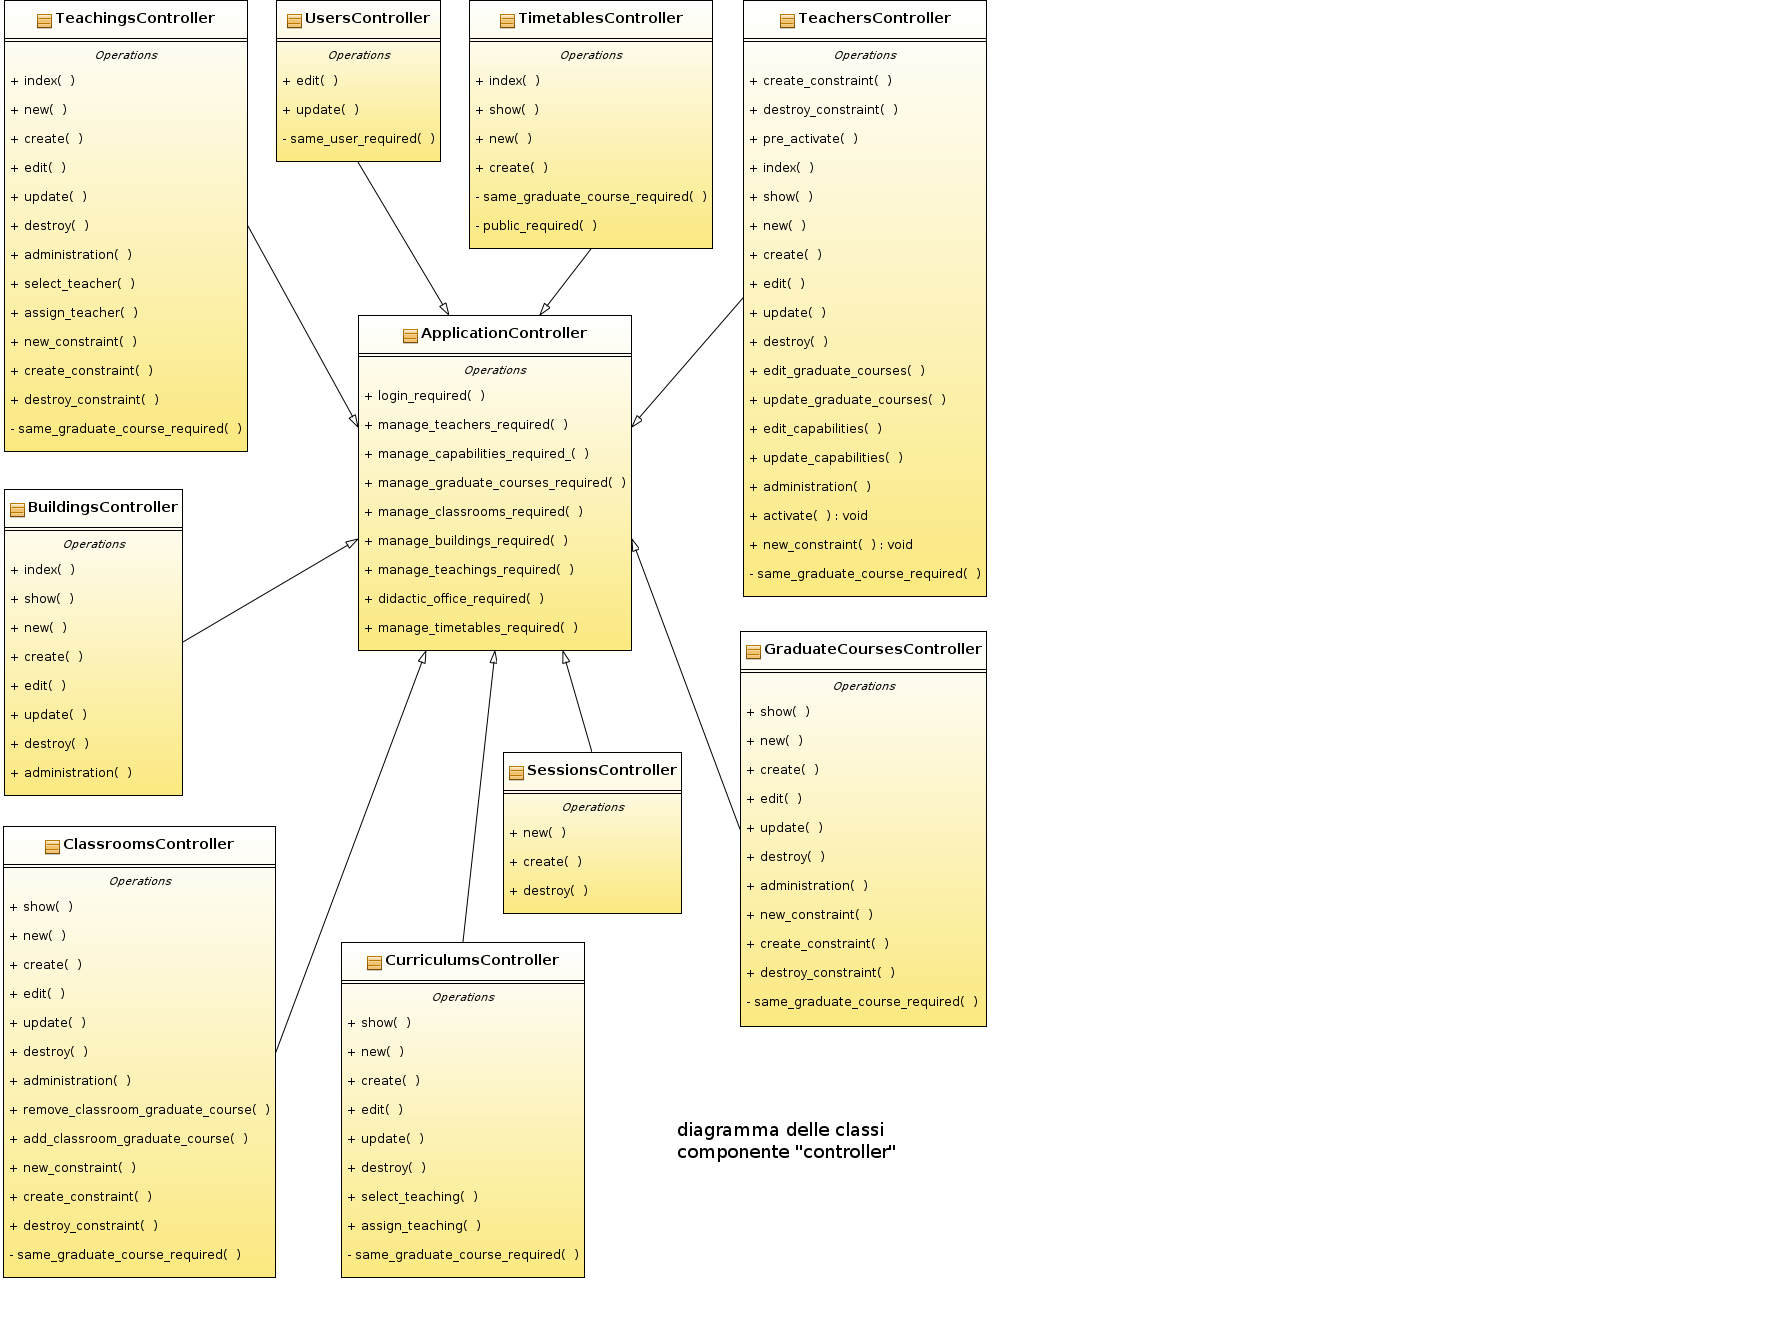
\includegraphics[scale=0.34]{images/Controller_ClassDiagram.png}
\subsubsection{Azioni comuni a più controller}
Per evitare fastidiose ripetizioni in questa sezione verranno descritti i metodi che figurano con lo stesso nome in diversi controller. La scelta dello stesso nome non è casuale, in quanto rispecchia la funzione dell'azione.
\begin{itemize}
 \item \verb|index|: rende disponibile alla view specifica un insieme d'istanze ed è raggiungibile eseguendo una richiesta GET all'indirizzo /nomecontroller. Ad esempio l'azione \verb|index| di \verb|GraduateCourseController| fornisce alla view un insieme di corsi di laurea ed è raggiungibile attraverso una richiesta GET all'indirizzo /graduate\_courses.
 \item \verb|show|: rende disponibile alla view specifica un'istanza ed è raggiungibile eseguendo una richiesta GET all'indirizzo /nomecontroller/id. Usando sempre l'esempio dei corsi di laurea, eseguendo una richiesta GET all'indirizzo /graduate\_courses/1 verranno visualizzate le informazioni relative al corso di laurea con id 1.
 \item \verb|new|: rende disponibile alla view specifica un'istanza vuota per permettere l'inserimento di un nuovo oggetto. E' raggiungibile eseguendo una richiesta GET /nomecontroller/new
 \item \verb|create|: acquisisce i dati da una richiesta POST per salvare l'oggetto nel database attraverso il model. Solitamente i dati provengono da una form con metodo POST presente nella view per l'azione \verb|new|. E' possibile comunque invocare questa azione mediante una richiesta POST all'indirizzo /nomecontroller
 \item \verb|edit|: rende disponibile alla view specifica un'istanza esistente per permetterne la modifica. e' raggiungibile attraverso una richiesta GET all'indirizzo /nomecontroller/id/edit
 \item \verb|update|: acquisisce i dati da una richiesta PUT per aggiornare lo stato dell'oggetto nel database attraverso il model. Solitamente i dati provengono da una form con metodo PUT presente nella view per l'azione \verb|edit|. E' possibile comunque invocare questa azione mediante una richiesta PUT all'indirizzo /nomecontroller/id
 \item \verb|destroy|: distrugge l'oggetto attraverso il model. Questa azione viene invocata tramite una richiesta DELETE all'indirizzo /nomecontroller/id
 \item \verb|administration|: rende disponibile alla view specifica un insieme d'istanze per effettuarne l'amministrazione. Questa azione è raggiungibile attraverso una richiesta GET all'indirizzo \\ /nomecontroller/administration.
 \item \verb|new_constraint|: rende disponibile alla view specifica un'istanza per un vincolo od una preferenza per permetterne l'inserimento. E' raggiungibile eseguendo una richiesta GET all'indirizzo \\ /nomecontroller/id/new\_constraint
 \item \verb|create_constraint|: acquisisce i dati da una richiesta POST per salvare il vincolo o la preferenza nel database attraverso il model. Solitamente i dati provengono da una form con metodo POST presente nella view per l'azione \verb|new_constraint|. E' possibile comunque invocare questa azione mediante una richiesta POST all'indirizzo /nomecontroller/id/create\_constraint
 \item \verb|destroy_constraint|: distrugge l'oggetto attraverso il model. Questa azione viene invocata tramite una richiesta DELETE all'indirizzo /nomecontroller/id/destroy\_contraint/id
\end{itemize}
Solitamente non è necessaria l'autenticazione o il possesso di alcuni privilegi per eseguire le azioni \verb|index| e \verb|show|. Per quanto riguarda gli altri metodi, invece, può ritenersi necessaria l'autenticazione od il possesso di alcuni privilegi. Per ogni controller sarà descritto questo aspetto.
Differente invece è il caso del metodo \verb|same_graduate_course_required|, dichiarato privato nei controllers che lo implementano. Questo metodo non rispecchia un'azione, ma è utilizzato come filtro, ovvero è chiamato prima o dopo una determinata azione, per impedire la modifica o la cancellazione di un oggetto appartenente ad un corso di laurea diverso da quello dell'utente autenticato.
\subsubsection{ApplicationController}
Questa classe deriva direttamente da \verb|ActionController::Base|, ed è estesa da ogni controller. Prevede metodi di pubblica utilità per gli altri controller, ma nessuna azione. L' \verb|ApplicationController| del sistema Sigeol prevede i seguenti metodi pubblici, utilizzati come filtri dagli altri controller.
\begin{itemize}
 \item \verb|login_required|: se l'utente non è autenticato questo metodo reindirizza alla pagina di login
 \item \verb|manage_teachers_required|: se l'utente non possiede i privilegi per gestire i docenti questo metodo reindirizza alla pagina principale mostrando un errore.
 \item \verb|manage_capabilities_required|: se l'utente non possiede i privilegi per gestire i privilegi questo metodo reindirizza alla pagina principale mostrando un errore.
 \item \verb|manage_graduate_courses_required|: se l'utente non possiede i privilegi per gestire i corsi di laurea questo metodo reindirizza alla pagina principale mostrando un errore.
 \item \verb|manage_classrooms_required|: se l'utente non possiede i privilegi per gestire le aule questo metodo reindirizza alla pagina principale mostrando un errore.
 \item \verb|manage_buildings_required|: se l'utente non possiede i privilegi per gestire gli edifici questo metodo reindirizza alla pagina principale mostrando un errore.
 \item \verb|manage_teachings_required|: se l'utente non possiede i privilegi per gestire gli insegnamenti questo metodo reindirizza alla pagina principale mostrando un errore.
 \item \verb|manage_timetables_required|: se l'utente non possiede i privilegi per gestire gli orari questo metodo reindirizza alla pagina principale mostrando un errore.
 \item \verb|didactic_office_required|: se l'utente non appartiene ad una segreteria didattica questo metodo reindirizza alla pagina principale mostrando un errore.
\end{itemize}
\subsubsection{GraduateCoursesController}
Il controller \verb|GraduateCourseController| permette alla segreteria didattica di creare e eliminare i corsi di laurea. Inoltre permette agli utenti con gli opportuni privilegi di aggiornare le informazioni relative ai propri corsi di laurea.
I filtri utilizzati in questo controller vengono tutti anteposti alle azioni e sono i seguenti:
\begin{itemize}
 \item \verb|login_required| non è utilizzato nelle azioni \verb|index| e \verb|show|
 \item \verb|manage_graduate_courses_required| è utilizzato nelle azioni \verb|edit|, \verb|update|, \verb|destroy|, \verb|administration|
 \item \verb|didactic_office_required| è utilizzato nelle azioni \verb|new|, \verb|create| e \verb|destroy|
 \item \verb|same_graduate_course_required| è utilizzato nelle azioni \verb|edit|,\\ \verb|update|, e \verb|destroy|.
\end{itemize}
\subsubsection{CurriculumsController}
Il controller \verb|CurriculumsController| permette all'utente con gli opportuni privilegi di creare, modificare ed eliminare le informazioni relative ai curricula dei propri corsi di laurea, nonchè di aggiungere o rimuove insegnamenti da quest'ultimi attreverso i metodi \verb|select_teaching|, raggiungibile medianta una richiesta GET all'indirizzo /curriculums/id/select\_teaching, e \verb|assign_teaching|, raggiungibile mediante una richiesta POST all'indirizzo /curriculums/id/assign\_teaching. Il primo fornisce alla view una lista degli insegnamenti presenti nel corso di laurea a cui il curriculum appartiene, mentre il secondo crea questa associazione tramite il model.
I filtri utilizzati in questo controller vengono tutti anteposti alle azioni e sono i seguenti:
\begin{itemize}
 \item \verb|login_required| non è utilizzato solamente nell'azione \verb|show|
 \item \verb|manage_graduate_courses_required| non è utilizzato solamente nell'azione \verb|show|
 \item \verb|same_graduate_course_required| è utilizzato nelle azioni \verb|edit|,\\ \verb|update|, \verb|select_teaching| e \verb|assign_teaching|.
\end{itemize}
\subsubsection{UsersController}
Il controller \verb|UsersController| dispone solamente delle azioni \verb|edit| e \verb|update| e del metodo privato \verb|same_user_required| (utilizzato come filtro anteposto alle due azioni assieme al filtro \verb|login_required|). Questa scelta progettuale deriva dalla relazione tra i model \verb|Teacher|, \verb|DidacticOffice| e \verb|User|. Confrontare la sezione \ref{model}.
Il metodo privato \verb|same_user_required| garantisce che non si stia cercando di modificare un utente diverso dal proprio.
\subsubsection{TeachersController}
Il controller \verb|TeachersController| permette all'utente con gli opportuni privilegi di creare, modificare ed eliminare i docenti dei propri corsi da laurea, nonchè di attribuire ad essi nuovi privilegi e corsi di laurea. Attraverso l'azione \verb|new| viene rischiesto un indirizzo e-mail di un docente e l'azione \verb|create| verificherà se questo è presente o meno nel database. Nel primo caso se il docente appartiene già a quel corso di laurea verrà segnalato un errore, altrimenti verrà aggiunto; nel secondo caso verrà inviata al nuovo docente una mail con le istruzioni per la registrazione al sistema. Il nuovo docente tramite l'azione \verb|pre_activate|, raggiungibile mediante una richista GET all'indirizzo /teachers/id/pre\_activate?digest=, potrà completare la creazione dello proprio user, e del relativo indirizzo, che sarà delegata all'azione \verb|activate|, raggiungibile mediante una richiesta POST all'indirizzo /teachers/id/activate?digest=. La certezza che solamente il docente invitato potrà creare il proprio account è resa possibile tramite il parametro \verb|digest| che solamente chi ha ha ricevuto la mail di invito può conoscere.

Infine attraverso le azioni \verb|edit_graduate_courses|, \verb|edit_capabilities|, \verb|update_graduate_courses| e \verb|update_capabilities|, raggiungibili rispettivamente mediante una richiesta GET all'indirizzo \\ /teachers/id/edit\_graduate\_courses o /teachers/id/edit\_capabilities e mediante una richiesta POST all'indirizzo /teachers/is/update\_graduate\_courses o /teachers/id/update\_capabilities, è possibilile modificare o rimuovere corsi di laurea e privilegi ai docenti da user che ne hanno la facoltà.
I filtri utilizzati in questo controller vengono tutti anteposti alle azioni e sono i seguenti:
\begin{itemize}
 \item \verb|login_required| non è utilizzato nelle azioni \verb|index|, \verb|show| ed \verb|activate|
 \item \verb|manage_teachers_required|  è utilizzato nelle azioni \verb|new|, \verb|create|,\\ \verb|administration|, \verb|edit_graduate_courses|, \verb|update_graduate_courses|
 \item \verb|manage_capabilities_required| è utilizzato nelle azioni \\ \verb|edit_capabilities| e \verb|update_capabilities|
 \item \verb|same_graduate_course_required| è utilizzato nelle azioni \\ \verb|edit_graduate_courses|, \verb|edit_capabilities|,\\ \verb|update_graduate_courses| e \verb|update_capabilities|.
\end{itemize}
\subsubsection{SessionsController}
Il controller \verb|SessionsController| permette la creazione di una sessione al momento dell'autenticazione dello user. Utilizza quindi le azioni \verb|new|, \verb|create| e \verb|destroy| senza alcun filtro, raggiungibili rispettivamente con una richiesta GET all'indirizzo /session/new, POST all'indirizzo /session e DELETE all'indirizzo /session/id.
\subsubsection{TeachingsController}
Il controller \verb|TeachingsController| permette all'utente con gli opportuni privilegi di creare, modificare ed eliminare le informazioni relative agli insegnamenti dei propri corsi di laurea, nonchè di aggiungere o rimuove il docente che tiene l'insegnamento in questione attraverso le azioni \verb|select_teacher|, raggiungibile medianta una richiesta GET all'indirizzo \\ /teachings/id/select\_teacher, e \verb|assign_teacher|, raggiungibile mediante una richiesta POST all'indirizzo /teachers/id/assign\_teacher. Il primo fornisce alla view una lista dei docenti presenti nel corso di laurea a cui il curriculum appartiene, mentre il secondo crea questa associazione tramite il model.
I filtri utilizzati in questo controller vengono tutti anteposti alle azioni e sono i seguenti:
\begin{itemize}
 \item \verb|login_required| non è utilizzato nelle azioni \verb|index| e \verb|show|
 \item \verb|manage_teachings_required| non è utilizzato nelle azioni \verb|index| e \verb|show|
 \item \verb|same_graduate_course_required| è utilizzato nelle azioni \verb|edit|,\\ \verb|update|, \verb|destroy|, \verb|select_teacher| e \verb|assign_teacher|.
\end{itemize}
\subsubsection{BuildingsController}
Il controller \verb|BuildingsController| permette all'utente con gli opportuni privilegi di creare, modificare ed eliminare le informazioni relative agli edifici ed ai relativi indirizzi.
I filtri utilizzati in questo controller vengono tutti anteposti alle azioni e sono i seguenti:
\begin{itemize}
 \item \verb|login_required| non è utilizzato nelle azioni \verb|index| e \verb|show|
 \item \verb|manage_buildings_required| non è utilizzato nelle azioni \verb|index| e \verb|show|
\end{itemize}
Non è presente il filtro \verb|same_graduate_course_required| in quanto un edificio non appartiene ad uno o più corsi di laurea, bensì all'intero sistema universitario.
\subsubsection{ClassroomsController}
Il controller \verb|ClassroomsController| permette all'utente con gli opportuni privilegi di creare, modificare ed eliminare le informazioni relative alle aule, nonchè di aggiungere o rimuovere le aule ai propri corsi di laurea attraverso le azione \verb|add_classroom_graduate_course| e \\ \verb|remove_classroom_graduate_course| raggiungibili attraverso una richiesta POST agli indirizzi, rispettivamente,\\ /classrooms/id/add\_classroom\_graduate\_course e \\ /classrooms/id/remove\_classroom\_graduate\_course
I filtri utilizzati in questo controller vengono tutti anteposti alle azioni e sono i seguenti:
\begin{itemize}
 \item \verb|login_required| non è utilizzato solamente nell'azione \verb|show|
 \item \verb|manage_classrooms_required| non è utilizzato solamente nell' azione \verb|show|
 \item \verb|same_graduate_course_required| non è utilizzato nelle azioni \verb|show|, \verb|new| e \verb|create|
\end{itemize}
\subsubsection{TimetablesController}
Il controller \verb|TimetablesController| permette all'utente con gli opportuni privilegi di creare ed eliminare gli orari.
I filtri utilizzati in questo controller vengono tutti anteposti alle azioni e sono i seguenti:
\begin{itemize}
 \item \verb|login_required| non è utilizzato nelle azioni \verb|index| e \verb|show|
 \item \verb|manage_timetables_required| non è utilizzato nelle azione \verb|index| e \verb|show|
 \item \verb|same_graduate_course_required| non è utilizzato nelle azioni \verb|index|, \verb|show|, \verb|new|, \verb|create|
 \item \verb|public_required| è utilizzato nell'azione \verb|show| ed assicura che l'orario che si intente visualizzare sia stato dichiarato pubblico da un utente con gli opportuni privilegi.
\end{itemize}
\subsection{Componente View}
Il componente View si occupa di presentare le informazioni presenti nel sistema a chiunque le richieda, sia esso un utente finale o un altro sistema software. Per far ciò sono presenti diversi elementi in questa componente, tra i quali:
\begin{itemize}
 \item Layouts: impostano l'impaginazione e la struttura dei template.
 \item Templates: vengono incorporati in un layout e si occupano della effettiva presentazione delle informazioni
 \item Partials: vengono incorporati in uno o più template o in uno o più layout. Sono frammenti di codice che presentano un sottoinsieme delle informazioni del sistema, riutilizzabili da più view.
\end{itemize}
\subsubsection{Layouts}
Il sistema Sigeol prevede un unico layout XHTML per tutta l'applicazione in modo da garantire la stessa impaginazione per ogni template. Come nella maggior parte dei siti web moderni è prevista un'intestazione, un \underline{footer}, un menu presente nella parte sinistra della pagina ed un blocco dei contenuti presenti nella parte centrale dove verranno renderizzati i template. In aggiunta sarà presente un menu di amministrazione ove richiesto che verrà collocato nella parte superiore del blocco dei contenuti.

Di seguito è riportata una immagina esplicativa della struttura del layout:

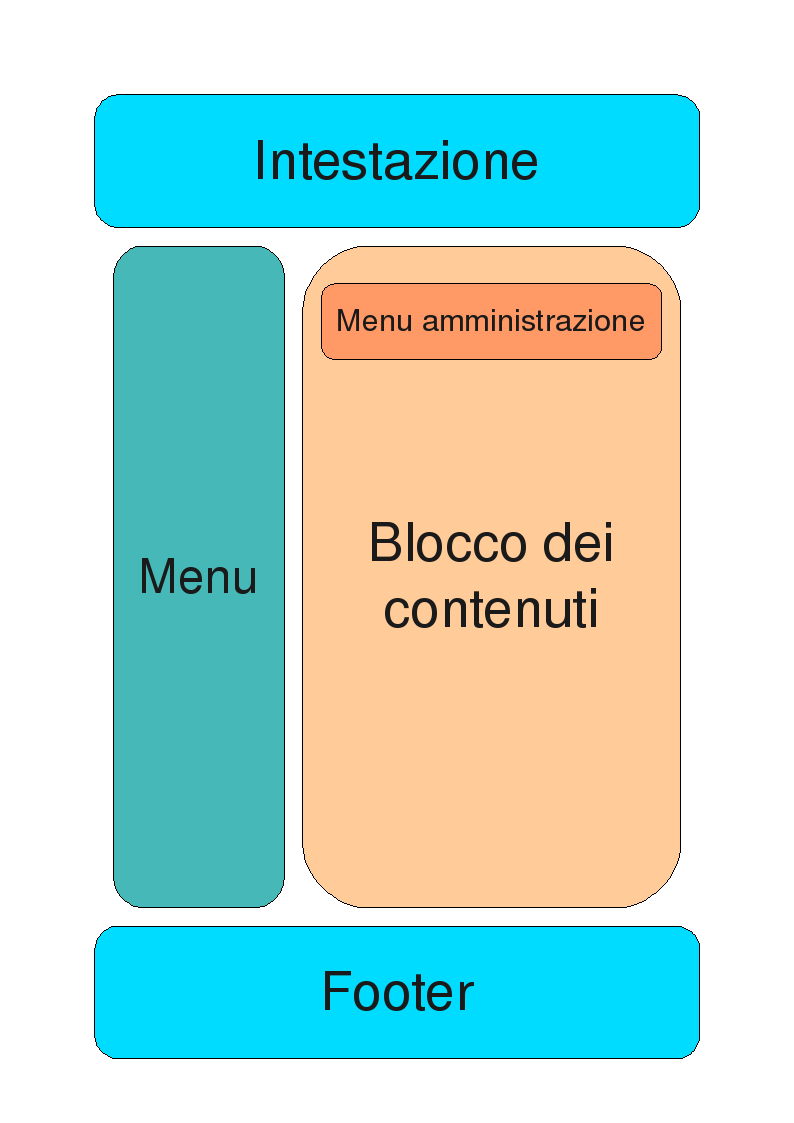
\includegraphics[scale=0.50]{images/layout.png}
\subsubsection{Templates}
Il sistema Sigeol prevede un diverso template per ogni azione raggiungibile attraverso una richiesta GET presente in ogni controller. Di seguito viene riportata una descrizione di ogni template:
\subsubsection*{Template comuni a più controller}
Per evitare fastidiose ripetizione di seguito sono riportate le descrizioni dei template per le azioni che figurano in più controller:
\begin{itemize}
 \item \verb|new.html.erb|: presenta un form per l'inserimento di una nuova istanza.
 \item \verb|edit.html.erb|: presenta un form per la modifica di un'istanza esistente.
 \item \verb|index.html.erb|: presenta un elenco ordinato di un insieme di istanze.
 \item \verb|show.html.erb|: presenta le informazioni relativa ad una determinata istanza.
 \item \verb|administration.html.erb|: presenta un elenco ordinato di un insieme di istanza e le relative funzioni
 per amministrarle.
 \item \verb|new_constraint.html.erb|: presenta un form per l'inserimento di un nuovo vincolo o preferenza
\end{itemize}
Inoltre per garantire l'interoperabilità dei dati sono presenti i template XML per tutte le azioni \verb|index| e \verb|show|, nonchè un template PDF per l'azione \verb|show| di \verb|TimetablesController|.
\subsubsection*{Template per TeachingsController}
Il template XHTML \verb|select_teacher.html.erb| è presente per il \\ \verb|TeachingsController| per l'azione \verb|select_teacher|.  Questo presenta un form per l'assegnamento di un docente ad un insegnamento utilizzando metodi per la presentazione automatica della lista dei docenti come i tag XHTML \verb|<select>| e \verb|<option>|.
\subsubsection*{Template per CurriculumsController}
Il template XHTML \verb|select_teaching.html.erb| è presente per il \\ \verb|CurriculumsController| per l'azione \verb|select_teaching|.  Questo presenta un form per l'assegnamento di un insegnamento ad un curriculum utilizzando metodi per la presentazione automatica della lista degli insegnamenti come i tag XHTML \verb|<select>| e \verb|<option>|.
\subsubsection*{Template per TeachersController}
Il \verb|TeachersController| prevede diverse azioni raggiungibili attraverso una richiesta GET ed i relativi template XHTML sono i seguenti:
\begin{itemize}
 \item \verb|pre_activate.html.erb|: presenta un form per l'attivazione dello \verb|user| del docente invitato
 \item \verb|edit_capabilities.html.erb|: presenta un form per l'assegnazione di nuovi privilegi allo \verb|user| detenuto dal docente utilizzando metodi per la presentazione automatica della lista dei privilegi come li tag XHTML \verb|<input type="checkbox">|
 \item \verb|edit_graduate_courses.html.erb|: presenta un form per l'assegnazione di nuovi corsi di laurea allo \verb|user| dtenuto dal docente utilizzando metodi per la presentazione automatica della lista dei corsi di laurea come i tag XHTML \verb|<select>| e \verb|<option>|
\end{itemize}
\subsubsection{Partials}
Il sistema Sigeol prevede l'uso di partials per la visualizzazione delle informazioni che sono riutilizzate in più view. Ognuno di essi è caratterizzato dalla presenza di un \_ (underscore) prima del nome del file che sono della forma \verb|_show_nomemodel.html.erb| e \verb|_show_nomemodel_admin.html.erb| e dovranno essere contenuti nella rispettiva directory che contiene i template del controller associato a \verb|nomemodel| (ad esempio \verb|_show_teaching.html.erb| è contenuto all'interno della directory \verb|app\views\teachings|. I partial del primo tipo visualizzano le informazioni dell'oggetto di tipo \verb|nomemodel| per le azioni di pubblico accesso, mentre i secondi per le azioni di amministrazione con le relative funzioni.

Per i controller che presentano l'azione \verb|administration| e necessitano di un menu di amministrazione è presente un partial \verb|_menu_admin.html.erb| per la visualizzazione del suddetto menu che risiederà nella stessa directory che contiene i template del controller in questione.

I partials, infine, che vengono utilizzati dal layout sono contenuti nella directory \verb|app\views\shared|, come ad esempio \verb|_user_sidebar.html.erb|.
\subsection{Componente Helper}\label{helper}
Il componente Helper si occupa di raccogliere le funzionalità di utilità necessarie ai componenti del pattern MVC. Ogni file che rappresenta un Helper non conterrà una classe, bensì un modulo, ovvero un insieme di metodi di pubblica utilità. Per ogni controller è previsto lo specifico Helper, anche se non è necessario che siano presenti dei metodi in quanto non tutti i controller (e le rispettive view) necessitano di funzioni ausiliarie.
\subsubsection{ApplicationHelper}
L' \verb|ApplicationHelper| contiene i metodi di utilità che non trovano una collocazione logica negli altri helper, nonchè tutte le funzionalità ausiliare richieste da più classi delle diverse componenti.
I metodi presenti all'interno dell' \verb|ApplicationHelper| sono i seguenti:
\begin{itemize}
 \item \verb|first_upper(name)|: metodo che restituisce la stringa \verb|name| a cui viene reso maiscolo il primo carattere e minuscoli i rimanenti.
 \item \verb|login_form|: metodo che \underline{renderizza} il partial per la form per il login.
 \item \verb|standard_sidebar|: metodo che renderizza il partial per il menu pubblico.
 \item \verb|user_sidebar|: metodo che renderizza il partial per il menu privato.
 \item \verb|link(user)|: metodo che restituisce l'insieme dei link disponibili per \verb|user|.
\end{itemize}
\subsubsection{BuildingsHelper}
I metodi presenti all'interno del \verb|BuildingsHelper| sono i seguenti:
\begin{itemize}
 \item \verb|menu_admin|: metodo che renderizza il partial per il menu di amministrazione per gli edifici.
 \item \verb|show_building_admin(building)|: metodo che renderizza il partial per l'amministrazione del \verb|building|.
 \item \verb|show_building(building)|: metodo che renderizza il partial per la visualizzazione del \verb|building|.
\end{itemize}
\subsubsection{ClassroomsHelper}
I metodi presenti all'interno del \verb|ClassroomsHelper| sono i seguenti:
\begin{itemize}
 \item \verb|menu_admin|: metodo che renderizza il partial per il menu di amministrazione per le aule.
 \item \verb|show_classroom_admin(classroom)|: metodo che renderizza il partial per l'amministrazione della \verb|classroom|.
\item \verb|show_classroom(classroom)|: metodo che renderizza il partial per la visualizzazione della \verb|classroom|.
\end{itemize}
\subsubsection{CurriculumsHelper}
I metodi presenti all'interno del \verb|CurriculumsHelper| sono i seguenti:
\begin{itemize}
\item \verb|show_curriculum_admin(curriculum)|: metodo che renderizza il partial per l'amministrazione del \verb|curriculum|.
\item \verb|show_curriculum(curriculum)|: metodo che renderizza il partial per la visualizzazione del \verb|curriculum|.
\end{itemize}
\subsubsection{SessionsHelper}
Non è presente nessun metodo all'interno di \verb|SessionsHelper|.
\subsubsection{GraduateCoursesHelper}
I metodi presenti all'interno del \verb|GraduateCoursesHelper| sono i seguenti:
\begin{itemize}
 \item \verb|menu_admin|: metodo che renderizza il partial per il menu di amministrazione per i corsi di laurea
 \item \verb|show_graduate_course_admin(graduate_course)|: metodo che renderizza il partial per l'amministrazione del  \verb|graduate_course|.
\item \verb|show_graduate_course(graduate_course)|: metodo che renderizza il partial per la visualizzazione del \verb|graduate_course|.
\end{itemize}
\subsubsection{TeachersHelper}
I metodi presenti all'interno del \verb|TeachersHelper| sono i seguenti:
\begin{itemize}
 \item \verb|menu_admin|: metodo che renderizza il partial per il menu di amministrazione per i docenti.
 \item \verb|show_teacher_admin(teacher)|: metodo che renderizza il partial per l'amministrazione del \verb|teacher|.
 \item \verb|show_teacher(teacher)|: metodo che renderizza il partial per la visualizzazione del \verb|teacher|.
\end{itemize}
\subsubsection{TeachingsHelper}
I metodi presenti all'interno del \verb|TeachingsHelper| sono i seguenti:
\begin{itemize}
 \item \verb|menu_admin|: metodo che renderizza il partial per il menu di amministrazione per gli insegnamenti.
 \item \verb|show_teaching_admin(teaching)|: metodo che renderizza il partial per l'amministrazione del \verb|teaching|.
 \item \verb|show_teaching(teaching)|: metodo che renderizza il partial per la visualizzazione del \verb|teaching|.
\end{itemize}
\subsubsection{TimetablesHelper}
I metodi presenti all'interno del \verb|TimetablesHelper| sono i seguenti:
\begin{itemize}
 \item \verb|menu_admin|: metodo che renderizza il partial per il menu di amministrazione per gli orari.
 \item \verb|show_timetable_admin(timetable)|: metodo che renderizza il partial per l'amministrazione del \verb|timetable|.
 \item \verb|show_timetable(timetable)|: metodo che renderizza il partial per la visualizzazione del \verb|timetable|.
\end{itemize}
\subsubsection{UsersHelper}
I metodi presenti all'interno del \verb|UsersHelper| sono i seguenti:
\begin{itemize}
 \item \verb|show_not_active_users(user)|: metodo che renderizza il partial per la visualizzazione dello \verb|user| non ancora attivo.
\end{itemize}
\subsection{Componente MiddleMan}
Il componente \verb|MiddleMan| viene utilizzato per effettuare esecuzioni (istantanee e/o schedulate) di calcolo dell'orario. \\ 
Esso implementa le seguenti operazioni:
\begin{itemize}
\item ricezione delle richieste, da parte dell'applicazione, di aggiunta di nuove date per la generazione dell'orario relativo ad uno specifico corso di laurea
\item assegnazione alla componente \verb|Algorithm| della generazione dell'orario relativo ad uno specifico corso di laurea
\item segnalazione all'applicazione della fine del calcolo 
\end{itemize}
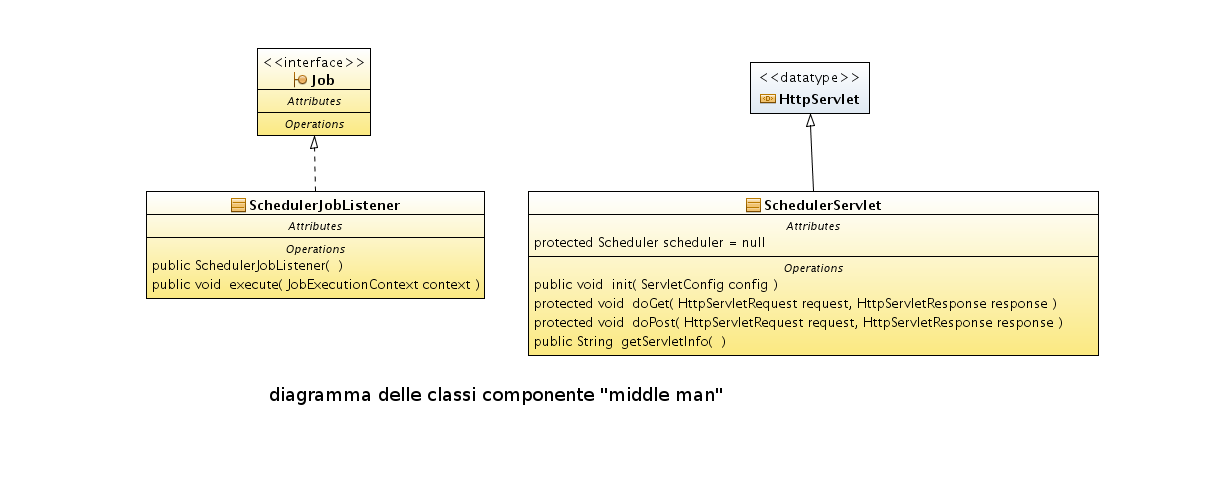
\includegraphics[scale=0.34]{images/MMserv_diagram_class.png}
\subsubsection{SchedulerServlet}
Servlet che si occupa di ricevere le richieste (di tipo HTTP POST e GET) dall'applicazione:
\begin{description}
\item[POST] \\ 
Parametri: course, date \\
crea una nuovo trigger che si attiverà alla data (date) per il corso di laurea (course) specificato 
\item[GET] \\ 
Parametri: course, inputfile, timeout \\
viene inizializzata ed eseguita la componente \verb|Algorithm| con i parametri ricevuti
\end{description}
\subsubsection{SchedulerJobListener}
Classe che viene richiamata all'attivazione di un evento precedentemente schedulato (nel nostro caso la generazione dell'orario di un determinato corso di laurea ad una certa data).
Si occupa di segnalare all'applicazione l'attivazione del calcolo dell'orario del corso di laurea specificato  
\subsection{Componente Algorithm}
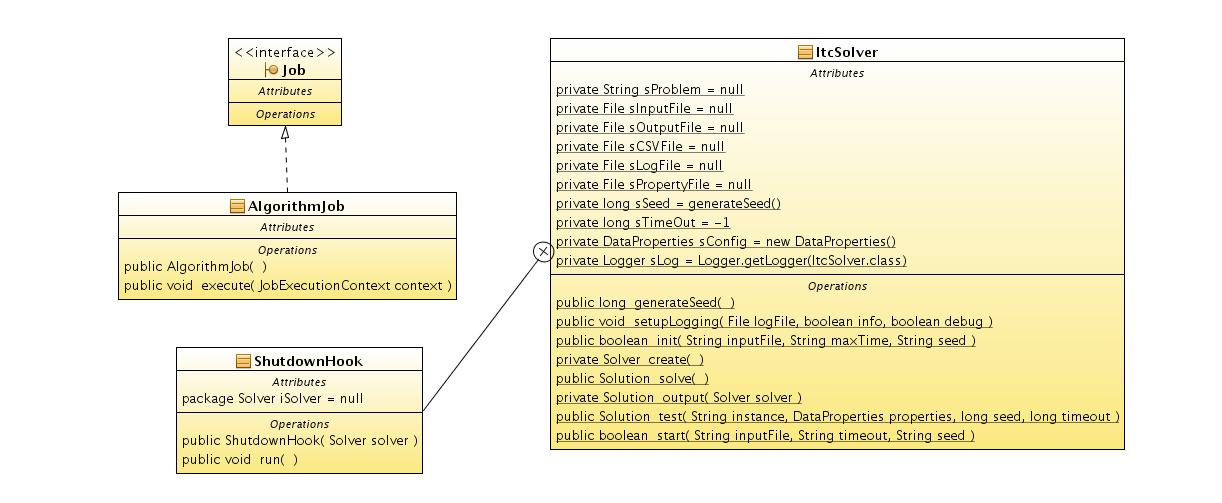
\includegraphics[scale=0.34]{images/MMalg_diagram_class.png}
\subsubsection{AlgorithmJob}
Ogni singola istanza della classe \verb|AlgorithmJob| esegue il calcolo dell'orario relativo ad un determianto corso di laurea.
\subsubsection{ItcSolver}
Classe che si occupa di leggere il file di input (contenente tutte le informazioni richieste relative al calcolo e generazione dell'orario) ed eseguire effettivamente l'algoritmo.
\newpage
\section{Organizzazione delle directories}
Per facilitare la comprensione dell'organizzazione del sistema Sigeol, viene presentata in questa sezione la struttura delle directories. Per un dettaglio maggiore dell'organizzazione si prega di far riferimento al sito ufficiale di Ruby on Rails. Nella figura che segue viene illustrata la gerarchia \\
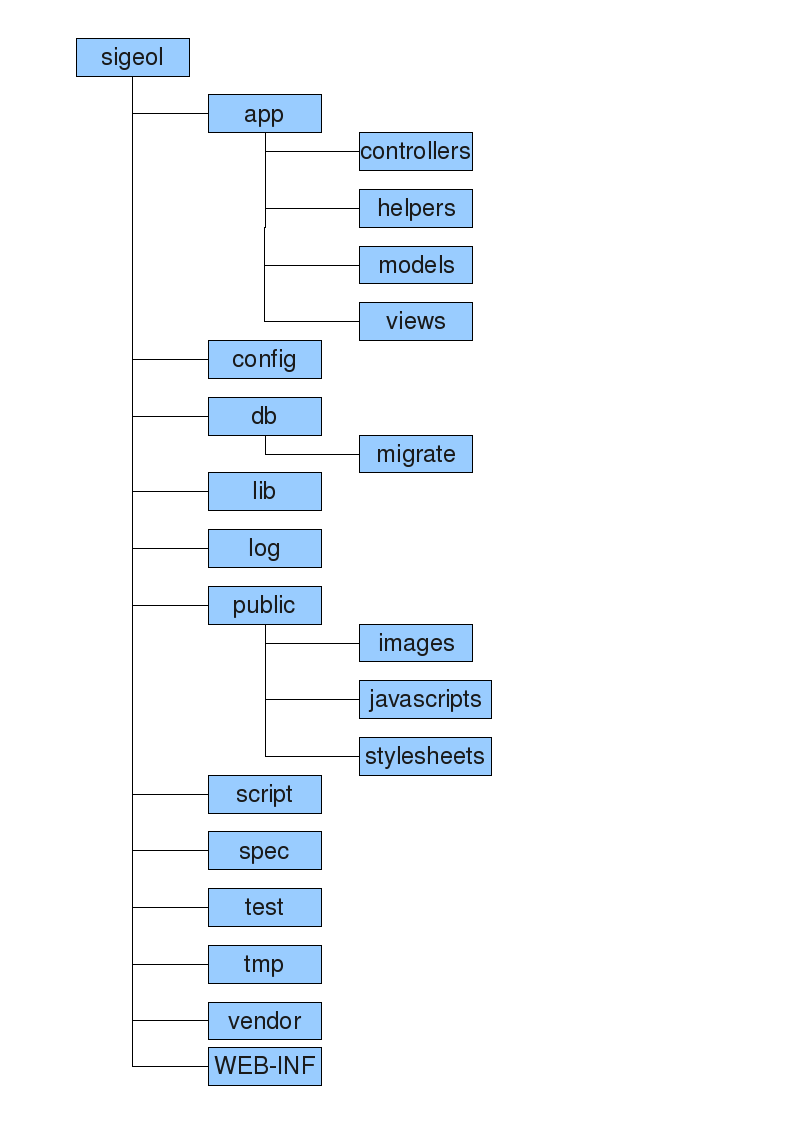
\includegraphics[scale=0.59]{images/gerarchiacartelle.png}
A differenza delle consuete applicazioni sviluppate tramite il framework Rails, il sistema Sigeol presente la cartella \verb|WEB-INF| che contiene tutte le classi e librerie utilizzate dalla servlet e il suo file di configurazione web.xml.\\ Per ulteriori informazioni sulla tecnologia servlet visitare il sito http://java.sun.com/products/servlet/ .
\modifiche
\end{document}
